\documentclass[border=10pt]{standalone}
\usepackage{fontspec}
\directlua{luaotfload.add_fallback("hmbfallback",{"Noto Serif CJK TC:mode=node;","Noto Serif CJK JP:mode=node;","Noto Serif CJK SC:mode=node;"})}
\setmainfont{Noto Serif}[RawFeature={fallback=hmbfallback}]
\setsansfont{Noto Sans}[RawFeature={fallback=hmbfallback}]
\setmonofont{Noto Sans Mono}[RawFeature={fallback=hmbfallback}]
\tracinglostchars=3
\directlua{
local hmblog = function(n, p) texio.write_nl("log", "HMB-SANDBOX-VIOLATION " .. n .. " " .. tostring(p)) end
local hmbin = function(p) return type(p) == "string" and (string.sub(p, 1, 5) == "/job/" or (not (string.sub(p, 1, 1) == "/") and not string.find(p, "..", 1, true))) end
local hmbblock = function(t, n) if t and t[n] then t[n] = function(...) hmblog(n, (...)); return nil, "blocked" end end end
local hmbpath = function(t, n) if t and t[n] then local f = t[n]; t[n] = function(p, ...) if not hmbin(p) then hmblog(n, p) end; return f(p, ...) end end end
hmbblock(os, "execute"); hmbblock(os, "exec"); hmbblock(os, "spawn"); hmbblock(io, "popen")
hmbpath(os, "remove"); hmbpath(os, "rename"); hmbpath(lfs, "mkdir"); hmbpath(lfs, "rmdir"); hmbpath(lfs, "touch"); hmbpath(lfs, "link"); hmbpath(lfs, "chdir")
local hmbopen = io.open
io.open = function(p, m, ...) if type(m) == "string" and string.find(m, "[wa+]") and not hmbin(p) then hmblog("io.open-write", p) end; return hmbopen(p, m, ...) end
}

\usepackage{tikz}
\usetikzlibrary{calc}

\begin{document}
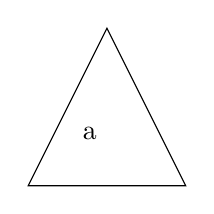
\begin{tikzpicture}
    % Define the vertices of the triangle.
    % Let the base be horizontal for simplicity in coordinates.
    % We can place the base on the x-axis.
    % Let the base length be 2 units for a simple representation.
    \coordinate (A) at (0, 0);
    \coordinate (B) at (2, 0);
    % The apex is centered above the base. Let the height be h.
    % For a general triangle, we can use a variable for the height,
    % but since the image only shows a label 'a' inside, we just need
    % to draw the triangle and place the label.
    \coordinate (C) at (1, 2); % Arbitrary height for visualization

    % Draw the triangle
    \draw (A) -- (B) -- (C) -- cycle;

    % Place the label 'a' inside the triangle.
    % The label 'a' appears to be placed near the center of the triangle,
    % perhaps near the centroid or just centrally located.
    % We will place it at the centroid for a standard representation.
    \coordinate (Centroid) at ($(A)!0.333!(B)!0.333!(C)$);

    % Draw the label 'a'
    \node at (Centroid) {a};
\end{tikzpicture}
\end{document}
